\documentclass[twoside,a4paper]{article}
\usepackage{geometry}
\geometry{margin=1.5cm, vmargin={0pt,1cm}}
\setlength{\topmargin}{-1cm}
\setlength{\paperheight}{29.7cm}
\setlength{\textheight}{25.3cm}

% useful packages.
\usepackage{float}
\usepackage{tikz}
\usetikzlibrary{calc}
\usetikzlibrary{arrows.meta}
\usepackage{pgfplots}
\usepackage{amsfonts}
\usepackage{amsmath}
\usepackage{amssymb}
\usepackage{amsthm}
\usepackage{enumerate}
\usepackage{graphicx}
\usepackage{multicol}
\usepackage{fancyhdr}
\usepackage{layout}
\usepackage{listings}
\usepackage{longtable}
\usepackage{multirow}
\usepackage{graphicx}
\usepackage{subfigure} 

% some common command
\newcommand{\dif}{\mathrm{d}}
\newcommand{\avg}[1]{\left\langle #1 \right\rangle}
\newcommand{\difFrac}[2]{\frac{\dif #1}{\dif #2}}
\newcommand{\pdfFrac}[2]{\frac{\partial #1}{\partial #2}}
\newcommand{\OFL}{\mathrm{OFL}}
\newcommand{\UFL}{\mathrm{UFL}}
\newcommand{\fl}{\mathrm{fl}}
\newcommand{\op}{\odot}
\newcommand{\Eabs}{E_{\mathrm{abs}}}
\newcommand{\Erel}{E_{\mathrm{rel}}}
\begin{document}

\tikzset{
  dot/.style={
    circle, fill=black, inner sep=1pt, outer sep=0pt
  },
  dot label/.style={
    circle, inner sep=0pt, outer sep=1pt
  }
  arrow1/.style = {
    draw = black, thick, -{Latex[length = 4mm, width = 1.5mm]},
  }
}

\pagestyle{fancy}
\fancyhead{}
\lhead{Liu jiyu (3170104256)}
\chead{Answer Document}
\rhead{2021.1}

TestPoint and TestAtomSpajor is very easy, the first is to test whether
we can get a point and the second is to test whether a segment is in
the interior of a Atom Spajor. So I will concentrate on the
remaining four test.
\section{TestSegment}

To determine the relative position of segments and determine the angle
between two segments, I use the segments as following:

\begin{center}
\begin{tikzpicture}[scale=0.75]
  \coordinate (o) at (0,0);
  \coordinate (A) at (1,4); \coordinate (B) at (4,4);
  \coordinate (C) at (1,3); \coordinate (D) at (4,5);
  \coordinate (E) at (2,4);  \coordinate (F) at (5,4);  
  \coordinate (G) at (1,5); \coordinate (H) at (5,5);
  \coordinate (I) at (1,2); \coordinate (J) at (2,5);

  \coordinate (A1) at (1,1); \coordinate (B1) at (-1,1);
  \coordinate (C1) at (1,0); 

  \draw[step=.5cm,gray!40,ultra thin](-2,-2) grid (6,6);
  \draw[<->] (-2,0) -- (0,0) -- (6,0);
  \draw[<->] (0,-2) -- (0,0) -- (0,6);
  
   \draw[red,ultra thick] (A) -- (B); \draw (C) -- (D);
   \draw (E) -- (B); \draw (E) -- (F); \draw (G) -- (H);
   \draw (I) -- (A); \draw (I) -- (G); \draw (E) -- (J);

   \draw[red,thick][->] (A1) -- (o);
   \draw[->] (o) -- (B1);
   \draw[->] (o) -- (C1);
   \draw[->] (o) -- (A1);
    \foreach \i/\angle in {A/-120, B/120, C/-80, D/120, E/60, F/-90,
      G/90, H/80, I/-95 ,J/90, A1/90 , B1/90 , C1/90,o/-130}  {
    \node[dot, label={[dot label]\angle:$\i$}] at (\i) {};
  }
 \end{tikzpicture}
\end{center}

The following picture is theresult of test program:

\begin{figure}[H]
  \begin{center}
  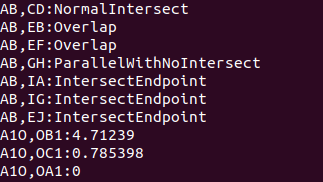
\includegraphics[height=5cm]{./pic/TestSegment.png}
  \caption{TestSegment}
  \end{center}
  \label{fig:figure1}
\end{figure}

\section{TestJordanCurve}

Curve1 is the curve1 of the panda, Curve2 is the curve1 of the mickey,
Curve3 is the curve2 of the panda. The test is to find the
intersection of the Curve1 and Curve2 and to judge whether Curve1
includes Curve3.

The following picture is theresult of test program:

\begin{figure}[H]
  \begin{center}
  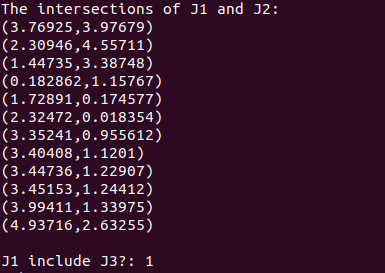
\includegraphics[height=5cm]{./pic/TestCurve.png}
  \caption{TestJordanCurve}
  \end{center}
  \label{fig:figure1}
\end{figure}

\section{TestPastingFunc}

\begin{center}
\begin{tikzpicture}[scale=0.45]
  \coordinate (o) at (0,0);
  \coordinate (A) at (2,5); \coordinate (B) at (3,0);
  \coordinate (C) at (2,-5); \coordinate (D) at (1,0);
  \coordinate (E) at (-2,5);  \coordinate (F) at (-1,0);  
  \coordinate (G) at (-2,-5); \coordinate (H) at (-3,0);
  \coordinate (I) at (-6,0); \coordinate (J) at (-4,-6);
  \coordinate (K) at (4,-6); \coordinate (L) at (6,0);

  \draw[step=.5cm,gray!40,ultra thin](-7,-7) grid (7,7);
  
  \draw[->] (A) -- (B) -- (C) -- (D) -- cycle;
  \draw[->] (E) -- (F) -- (G) -- (H) -- cycle;
  \draw[->] (A) -- (E) -- (I) -- (J) -- (K) -- (L) -- cycle;

  \fill[gray!40] (A)--(E)--(F)--(D)--cycle;
  \fill[gray!40] (E)--(I)--(J)--(K)--(L)--(A)--(B)
  --(C)--(D)--(F)--(G)--(H)--cycle;

  
    \foreach \i/\angle in {A/90, B/40, C/-80, D/60, E/60, F/120,
      G/-90, H/120, I/130 ,J/-90, K/-90, L/40,o/-90}  {
    \node[dot, label={[dot label]\angle:$\i$}] at (\i) {};
  }
 \end{tikzpicture}
\end{center}

The segment orientation is $A\rightarrow B \rightarrow C \rightarrow D
\rightarrow A \rightarrow E \rightarrow F \rightarrow G \rightarrow H
\rightarrow E \rightarrow I \rightarrow J \rightarrow J \rightarrow K
\rightarrow L \rightarrow A$.(I don't know why my tikz picture does
not show the arrow.) It is like the example of pasting function S2R-C
in the article.

Firstly, I will use a Segment vector which contains all segments in
the picture to initialize the Spajor,which means the Jordan Curve member in
the spajor is not a Jordan Curve. then I will cut and pasting function
to get a correct Spajor. 

The following is the result of test program.


\begin{figure}[H]
  \begin{center}
  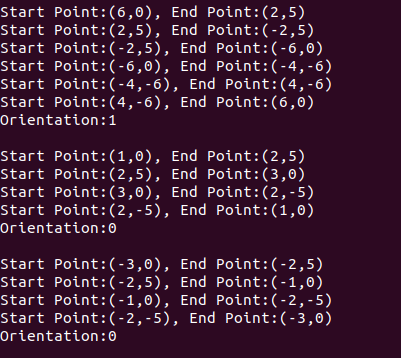
\includegraphics[height=6cm]{./pic/TestPasting.png}
  \caption{TestPasting}
  \end{center}
  \label{fig:figure1}
\end{figure}

\section{TestSpajor}

The last one is the acceptance test.

The following is the result of the test program, which returns three
.txt file, I use the result data to plot four pictures in Matlab:

\begin{figure}[htbp]
  \centering

  \subfigure[Initial Data]{
    \begin{minipage}{0.5\linewidth}
      \centering
      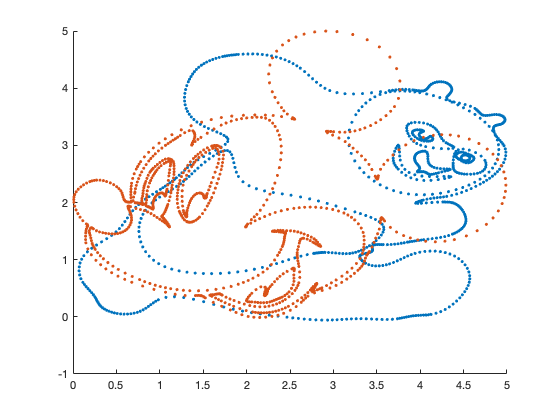
\includegraphics[height=7cm,width=7cm]{./pic/InitialData.png}
    \end{minipage}
  }
  \subfigure[Complementation of Panda]{
    \begin{minipage}{0.45\linewidth}
      \centering
      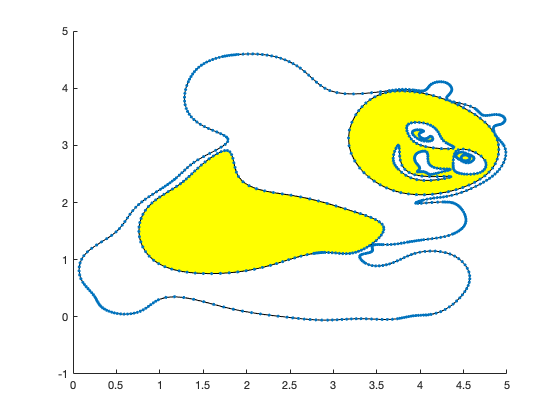
\includegraphics[height=7cm,width=7cm]{./pic/Complement_Result.png}
    \end{minipage}
  }
  
  \subfigure[Intersection of Mickey and Panda]{
    \begin{minipage}{0.5\linewidth}
      \centering
      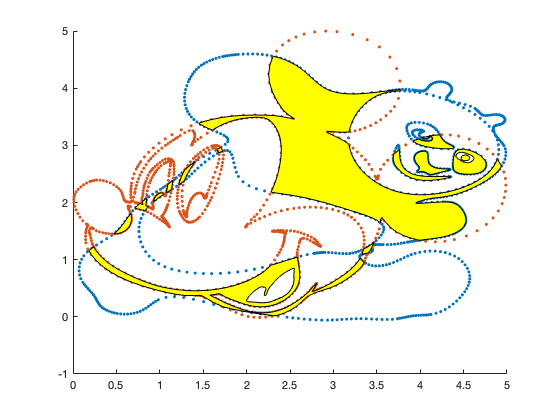
\includegraphics[height=7cm,width=7cm]{./pic/Meet_Result.png}
    \end{minipage}
  }
  \subfigure[Regularized Union of Mickey and Panda]{
    \begin{minipage}{0.45\linewidth}
      \centering
      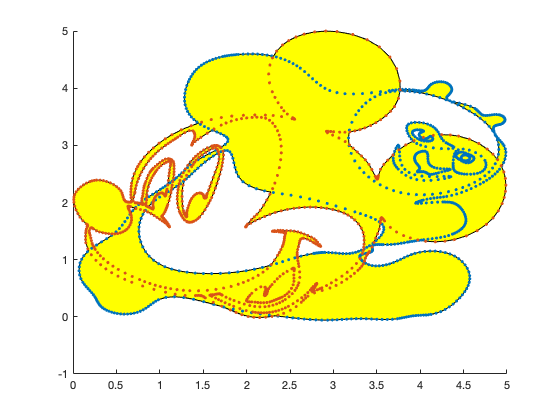
\includegraphics[height=7cm,width=7cm]{./pic/Join_Result.png}
    \end{minipage}
  }

  \centering
  \caption{TestSpajor}
\end{figure}




\end{document}


%%% Local Variables:
%%% mode: latex
%%% TeX-master: t
%%% End:
